
%In this section, I present the results of applying the classification methods described above.

\paragraph{Most comments result from mass-comment campaigns.}
Figure \ref{fig:comments-support} shows all comments posted on regulations.gov over time by whether they are exact or partial copies of another comment or not. While some agencies classify all duplicate comments as mass comments, I call comments that have between 2 and 99 identical copies, ``medium batch'' because such comments may reflect coordinated efforts among interest groups that do not include a public pressure strategy that involves mobilizing ordinary people. Here ``mass comments'' are comments that have either 100 or more identical copies or were uploaded in bulk batches of at least 100. This restrictive definition of what counts as mass engagement captures comments that were certainly mobilized by a campaign. As Figure \ref{fig:comments-support} shows mass commenting campaigns mobilize the vast majority of comments. In other words, most comments are from ordinary people.

\begin{figure}[h!]
    \centering
        \caption{Comments on Draft Rules Posted to Regulations.gov 2006-2018}
    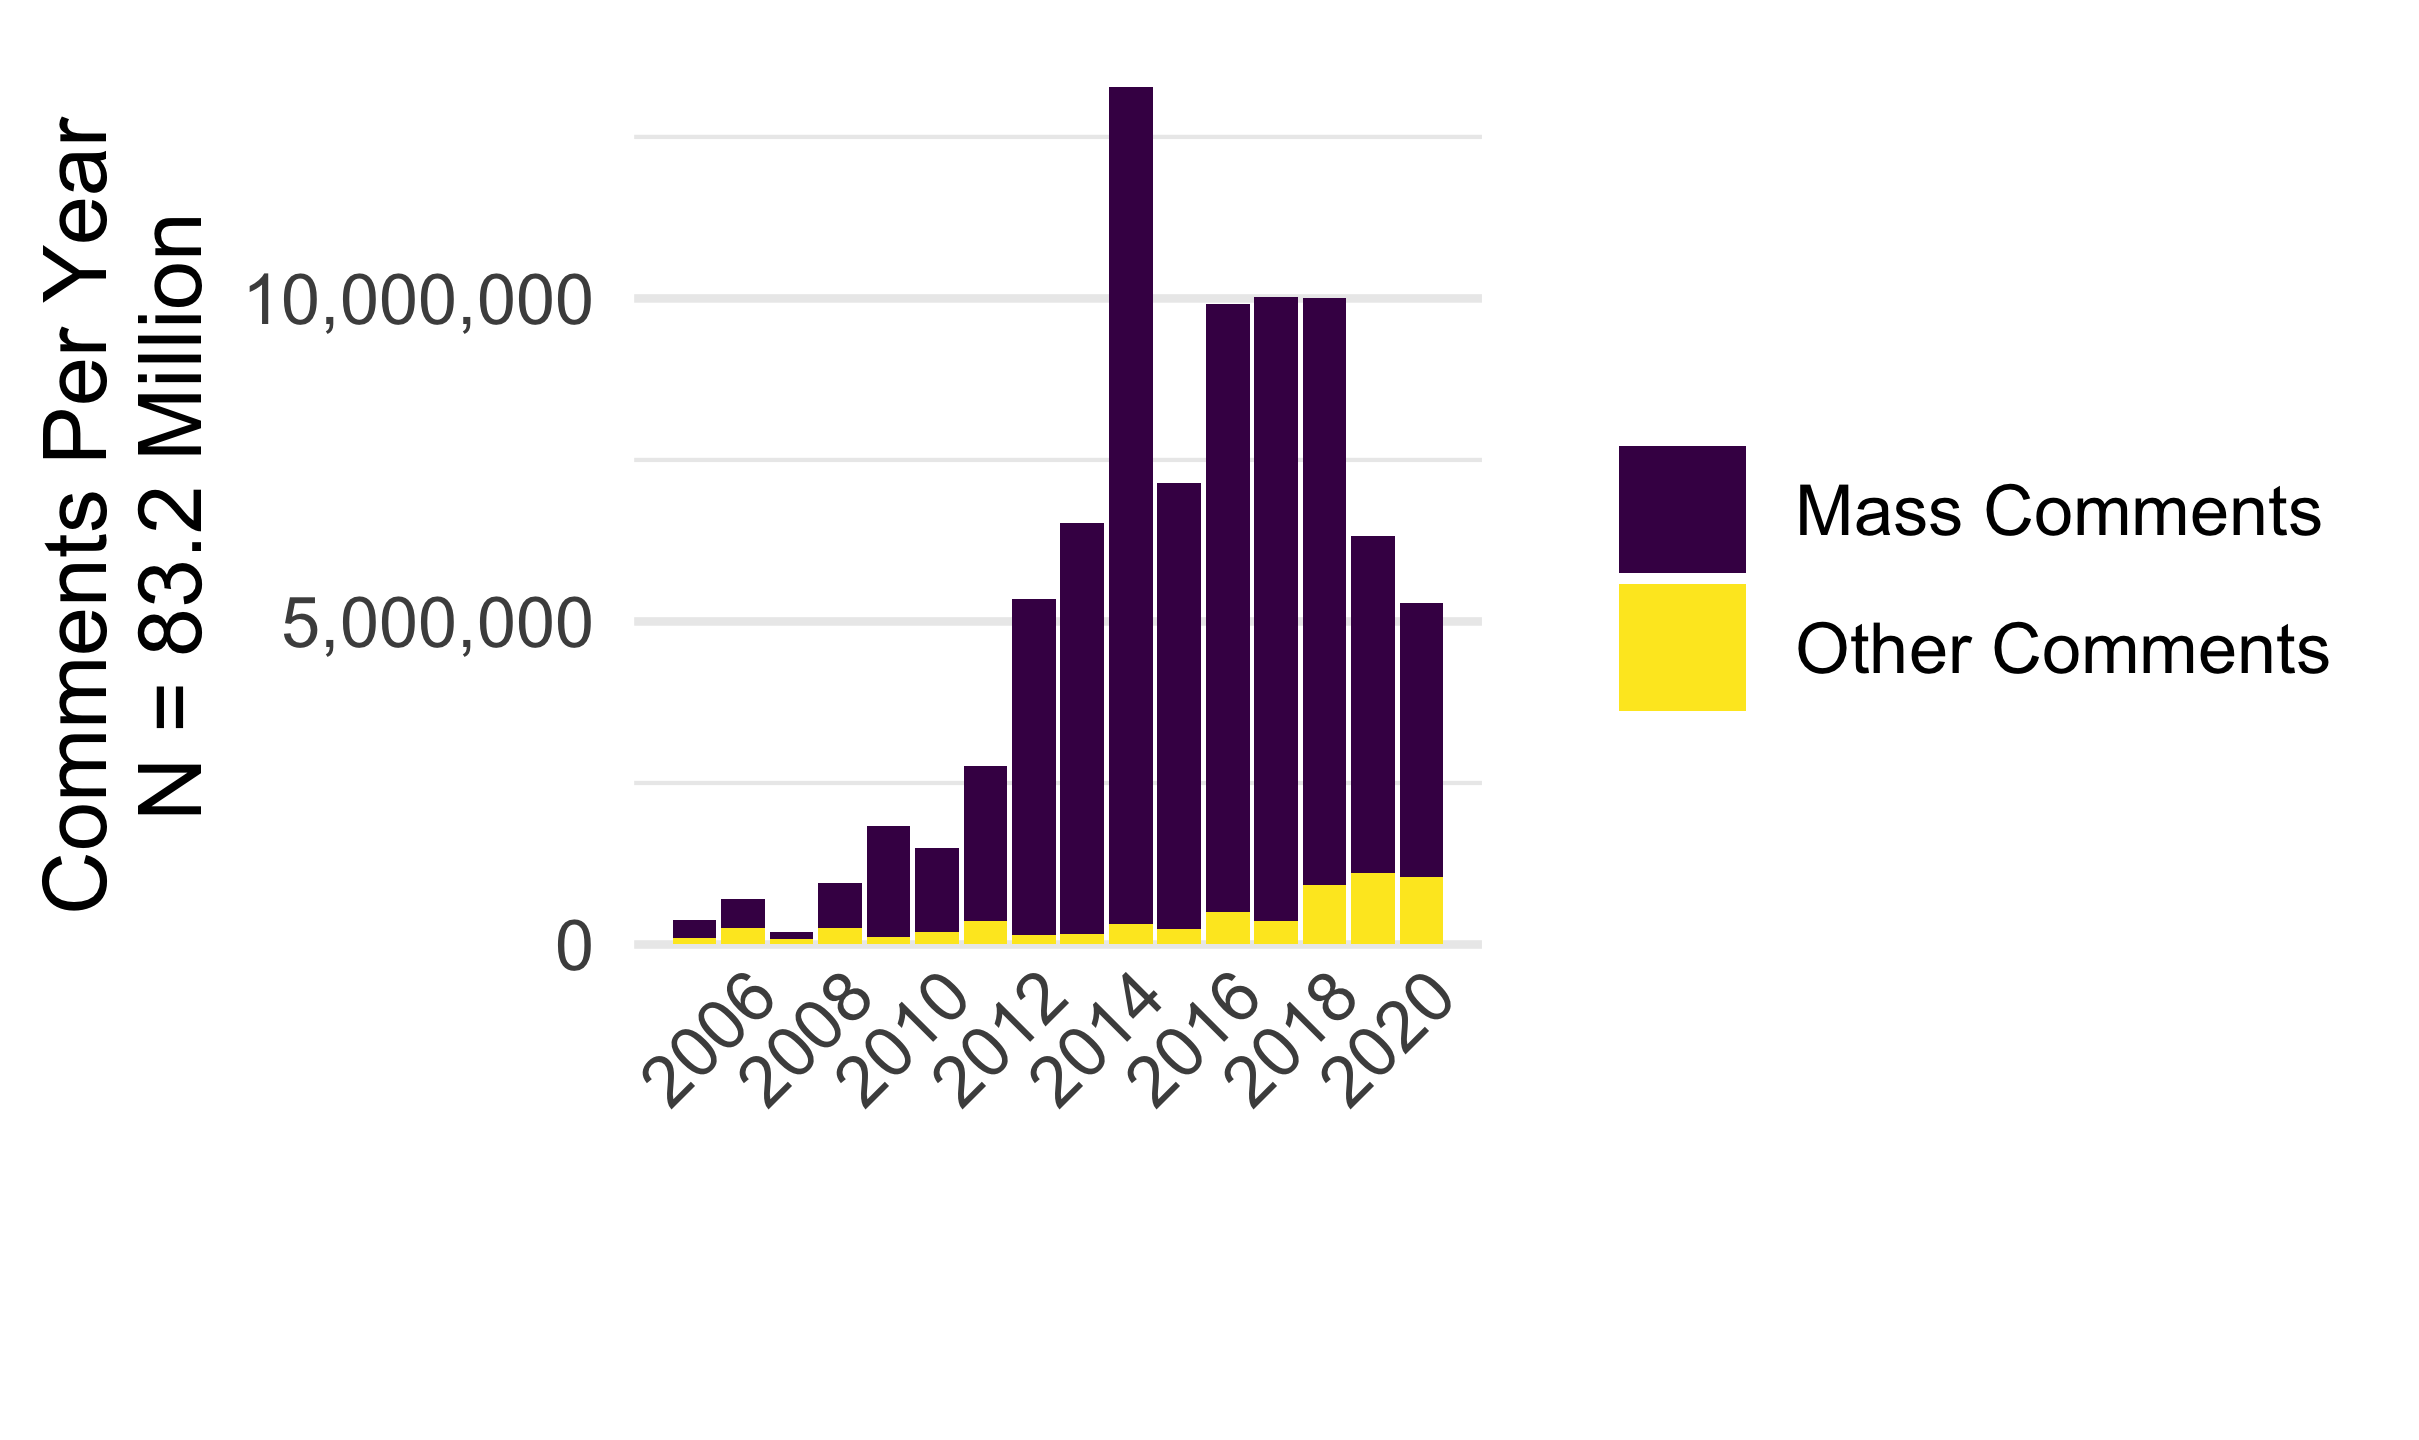
\includegraphics[height =2in]{Figs/comments-mass-1.png}
    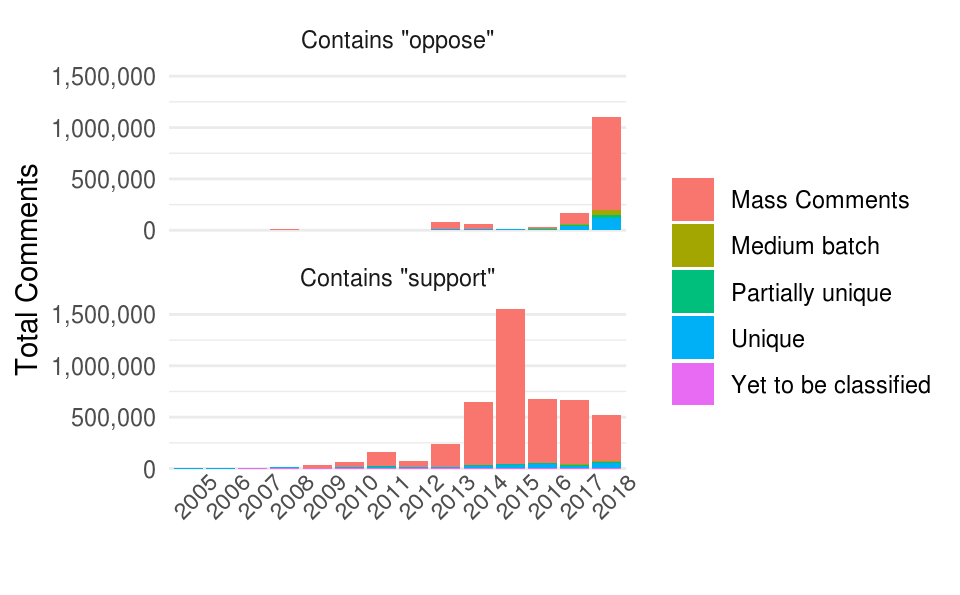
\includegraphics[height =2in]{Figs/comments-mass-support-vs-oppose-1.png}

    \label{fig:comments-support}
\end{figure}

The right pane of Figure \ref{fig:comments-support} shows results from a sample of several million comments for which I have digitized texts. Many of these comments appear to support proposed agency rules, as was the case with both the do not call and mercury rule examples. A rough measure of support (whether the comment text includes `` support '' or `` oppose '') shows that many more comments mention support, until 2018, when there is a fairly dramatic reversal in the share of comments mentioning ``support '' compared to those mentioning ``oppose '' (Figure \ref{fig:comments-support}). This may be a function of the changing regulatory agenda due to the change in presidential administration. 



\paragraph{Most comments occur on a small number of salient rules.} Approximately a third of public comments posted to regulations.gov were received on just ten regulations shown in figure \ref{fig:topdockets}.


\begin{figure}[h!]
    \centering
        \caption{Top 10 Dockets Receiving the Most Comments on regulations.gov and the top 20 Mobilizers}
    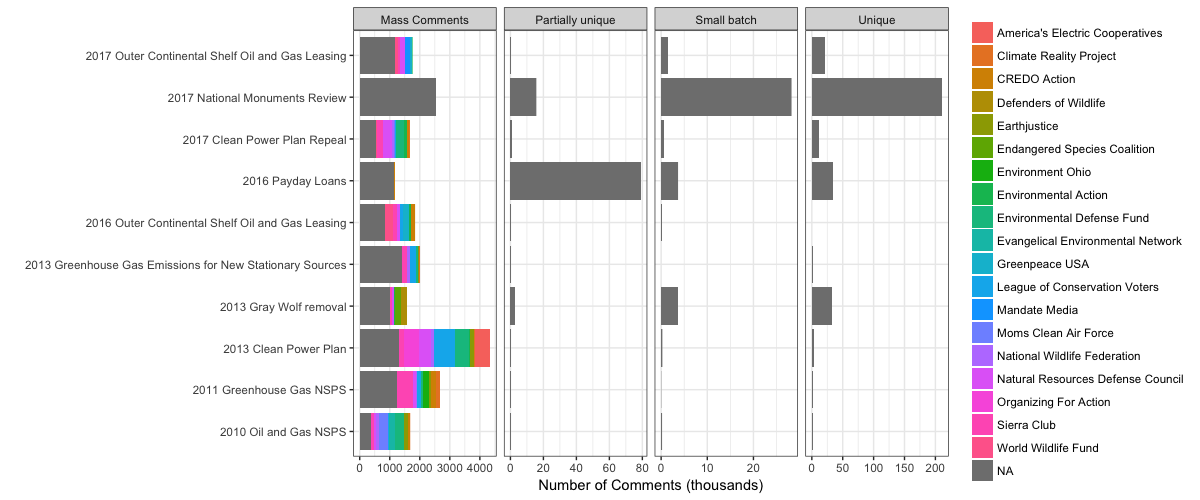
\includegraphics[width = 6in]{Figs/topdockets.png}
    \label{fig:topdockets}
\end{figure}


\paragraph{A coalition of public-interest organizations mobilize most comments.} As Figure \ref{fig:topdockets} % and \ref{fig:toporgs} 
shows, the most prolific mobilizers are environmental groups. On 5 out of the top 10 dockets (here including rulemaking and non-rulemaking dockets), a similar coalition of groups mobilized the majority of public comments. In part, this is because the Environmental Protection Agency produces a large share of the substantive rules posted to regulations.gov. However, it is notable that, on the top ten dockets, 19 of the top 20 mobilizers generally lobby together. America's Energy Cooperatives, an industry association, stands out as the lone mobilizer on behalf of material interest for its members. Notably, it only mobilized significantly on the Clean Power Plan but not on the subsequent Clean Power Plan repeal. 